\documentclass{./llncs2e/llncs}
\usepackage{graphicx}
%%%%
\usepackage{fixltx2e}
%%%%
\usepackage{mathtools}
%%%%
\usepackage[nolist,nohyperlinks]{acronym}
%%%%
\usepackage[section]{placeins}
%%%% Maintain images and tables within their respective sections
\usepackage{float}
%%%%
\usepackage[utf8]{inputenc}
%%%% Declare that we're using utf8 encoding
\usepackage{listings}
%%%% Include package for listings


% 
% Change the margins
% 
% \usepackage[margin=2.9cm]{geometry}

\begin{document}
\title{A Browser-based Interactive Development Environment for Generative Design}

%\subtitle{Your Thesis subtitle}
\author{Pedro Alfaiate, pedro.alfaiate@tecnico.ulisboa.pt}
\institute{Instituto Superior Técnico}

\maketitle

%----------------------------------------------------
%NAVabstract
\begin{abstract}
	Web technologies now allow distributed applications to be accessible without having to install anything more then a web browser.
	Apart from the features from desktop applications, web applications allow people to communicate and collaborate and also untie them from any particular computer.
	With modern web browser, interfaces are not limited to server generated web pages;
	they are now rivals of native desktop interfaces.
	\ac{gd} is in need of one such web application, an \ac{ide} in this case.
	
	In this report we will look at examples of both native and web applications and will use them as a basis for proposing a web based \ac{ide} for \ac{gd}.
\end{abstract}
%----------------------------------------------------
%NAVkeywords
\begin{keywords}
web browser, Generative Design, integrated development environment, javascript
\end{keywords}
%----------------------------------------------------
%NAVintroduction
\section{Introduction (2/3pgs)}
	%Introduce the power of programming.
	Programming is becoming an essential way of expressing ideas in a way a computer can understand them.
	Once a computer can understand an idea (or process) it can apply it as many times as we want.

	Expressing ideas or processes in a way a computer understands requires us to specify every detail of what we have in mind (sometimes too much) which forces us to really understand what they are.

	Many people have understood the power that comes from having a computer (or machine) doing lots of mechanical work and so have adopted programming as a new tool.

	%Introduce the need for IDEs. Introduce the demand for IDEs.
	Still, programming requires a lot of discipline from the programmer.
	He has to write the program in a programming language.
	He has to store it following a specific file structure.
	If he uses a specific \ac{api}, he will have to have its documentation at hand for quick reference.
	He may have to compile the program in order to run it.
	The compiler might detect syntactical errors that have to be corrected.
	If he notices that the program is misbehaving, he will have find the reason which normally involves starting the program and attaching a debugger to it.
	When he finds the reason, he will have to make corrections and test the program.
	And so on and so forth.

	All of this demands great time and effort from the programmer.
	All those small steps have to be learned and articulated by the programmer.
	It is an inevitably complex activity.
	And the programmer's productivity and enjoyment suffers from it.
	There has to be some way of lifting some of the work from the programmer.
	That is where \ac{ide}s come in.

	\ac{ide}s bring together all the tools needed while programming and automates all its small steps.
	They might do it so well that the programmer might forget that those steps still exist.
	We can imagine that novice programmers using these environments would simply be unaware of them.
	Programmers still have to write, run and debug their programs but they do so without losing time performing all those steps.
	And so \ac{ide}s have become essential to programming.
	
	%Go from software production IDEs to architecture specific IDEs.
	%Software development -> dynamic languages -> domain specific -> architecture specific
	There are \ac{ide}s dedicated to supporting software production, like Eclipse\cite{eclipse2007eclipse} and Visual Studio\cite{mvs2002mvs}.
	These \ac{ide}s support many programming languages and provide many tools needed for software production.
	They help programmers navigate big software projects and let them configure complex building processes.
	They also help them organizing the work on their software projects.
	They are good for large scale software projects but not as good for smaller projects such as making prototypes or merging programs together.
	They still require a lot of configuration before the programmer can start using them to make a program.
	Again, a programmer is being burdened with small steps that could be automated.
	This is where dynamic languages and their \ac{ide}s can be useful.

	%IDEs dynamic languages.
	\ac{ide}s for dynamic programming languages can go a step further in shortening the cycle between editing the program and seeing its effects.
	They allow programmers to quickly run their programs and provide ways to interact with them like \ac{repl}s.
	The programmer can now write his program and then start experimenting with it in the \ac{repl}, quickly testing some areas or quickly sketching new portions of the program.
	All this without having to write a separate program and compiling both.
	Dynamic languages themselves also play a part.
	They start to blur the line between programming language and programming environment.
	Being less strict and providing higher level concepts allows them to free programmers from having to state every detail of the program.
	They allow those missing details to be implicit.

	%IDEs domain specific.
	\ac{ide}s for dynamic languages are better but they are still too general.
	They stop at helping to program without covering problems specific to the bigger activities of their users, what they actually want to program.
	They don't automate the small repetitive steps present in activities where programming is used as a tool.
	\ac{ide}s like IPython and Impromptu are another step further.
	IPython helps scientists by providing them what is relevant to their work, such as automating gathering of data, transforming and visualizing it in order to draw conclusions.
	It integrates taking notes and programming.
	They no longer have to join the pieces of information into a single space, it is already done by the environment.
	Impromptu helps musicians to compose music procedurally.
	A musician using Impromptu doesn't have generate a MP3 file and then play it to actually hear what his program produced.
	He just starts his program and hears it.

	Here programming is no longer the main activity, it is used as a way to make computers do something we want.
	The results and ways to visualize (or hear) them are integrated into the environment.

	%IDEs architecture specific.
	As with scientists and musicians, architects can benefit from having \ac{ide}s specific to their programming needs.
	They can also benefit from automating small steps and integrating all tools needed to making their programs.
	In their case it requires a direct correspondence between the program and the 3D geometry that it creates.
	
	Following the trend of using programming in their work, architects started using programming to generate the 3D models of the buildings they are designing. 
	They use a process called \ac{gd}\cite{terzidis2003expressive,Maeda:2001:DN:559503}.
	By using \ac{gd}, they can easily create variants of their designs by changing a small set of parameters. 
	Those parameters are used by the computer to run the algorithm to generate an ``instance'' of their designs. \cite{Santos20144}

	There are several \ac{ide}s that make it easier to program for \ac{gd}. 
	%\footnote{In case of Generative Design it is a necessity to have a dedicated programming environment as architects may not be willing to program if it is too hard, too unknown.
	%After all, their work is not developing software, they will only program if it is a easier alternative for designing a building.}
	First, many \ac{cad} software packages used by architects have support for \ac{gd} provided by a plug-in or a set of plug-ins.
	In these software packages \ac{gd} is not the main way to model.
	Second, there are standalone programming environments like Processing\cite{reas2007processing} or Rosetta\cite{de2012modern}; the first is a programming environment for the visual arts and the second is an environment thought specifically for \ac{gd}. 
	As they come from textual programming community, these don't provide direct manipulation as a primary tool.

	Although these \ac{ide}s already enable architects to do \ac{gd} there is still room for improvement.
	They present some work on freeing architects from being stuck with one of the well established \ac{cad} software packages or one of their plug-ins.
	It is still possible to try to free them even further, they can be freed from the computer that runs their programs.

	One possibility for freeing them from the computer that runs their programs is moving the environment to the cloud and the web browser.

	%Architects also need to be independent from the CADs they are using.
	%It is often the case that they become experts in just one software.
	%They also become very dependent on that software.

	Web browser applications with heavy use of 3D graphics are now becoming common.
	There are 3D modeling applications, game editors and procedural 3D modeling applications.
	\footnote{Some examples are Clara.io\cite{houston2013clara}, a 3D modeling application, GooCreate\cite{goocreate2015site}, a game engine paired with a game editor, and OpenJSCAD\cite{openjscad2015site}, a procedural 3D modeling language with a browser based program editor.}
	These applications tend to be more independent from the details of the machine where they are running.
	They all share the same platform, the web browser.

	While there are some web browser applications where \ac{gd} can be applied there is still room for improving its support.
	As an example, OpenJSCAD lets programmers write and run programs that generate 3D objects and displays its results in an interactive 3D view.
	It doesn't provide constant feedback to changes when writing the program.
	The only way the programmer has to get feedback from the program is by explicitly running it.

	We propose a web browser based \ac{gd} environment. 
	Such environment will allow architects, or anyone interested in \ac{gd}, to edit \ac{gd} programs and visualize their results while not requiring any installation. 
	It will thus allow them to do \ac{gd} on any computer that has a modern browser. 
	Not being tied to a workstation will allow them to work closer to their clients and to more swiftly change their designs to accommodate the client's needs.

%----------------------------------------------------
%NAVobjectives
\subsection{Objectives (1pg)}
	The aim of this project is to provide architects and designers interested in creating 3D models with an environment that fosters the Generative Design approach while being accessible wherever there is a web browser and an internet connection.

	%Why does it need to be accessible wherever the architect is?
	Architects imagine buildings and will have to move their ideas outside of their heads wherever they are; if they don't, they might forget them forever. 
	We have to provide means to translate ideas and it has to be accessible wherever they are.

	How can we provide means to translate ideas? We make them translate the idea into a program, we encourage them to use Generative Design.

	When architects look for an environment to program they aren't looking for a software development \ac{ide} like Eclipse or Visual Studio. 
	They only need an environment where they can write their program and see the results. 
	All they want is accessible programming languages and environments.

	%TODO: Rephrase the following paragraph since the well established tools were introduced earlier.
	There are many well established tools that architects use to translate their ideas; 
	if we're going to come up with a solution that can rival them then \textbf{it must be as easy to try out as possible}; 
	and \textbf{be able to integrate with them}.
	%Should I say how it integrates with them? Which is by offering the possibility of producing effects on their current tools, more specifically the CADs they use.

	Summing up, the result of this project should:
	\begin{enumerate}
		\item Be accessible wherever the architect is working; \label{obj:access}
		\item Support the Generative Design approach; \label{obj:gen-design}
		\item Be as easy to try out as possible -- without a middle step to install it; \label{obj:no-install}
		\item Integrate with the tools that architects and designers already use.\label{obj:inter-op}
	\end{enumerate}


%----------------------------------------------------
%NAVrelatedwork
\section{Related Work (~17pgs)}

\subsection{IDE for GD}
	Developing and maintaining large software systems is a complex task.
	To deal with this complexity, software developers have many tools at their disposal and many of them are software themselves.
	Things like generating diagrams from source code (like class hierarchy diagrams and control-flow diagrams), source code versioning and management, testing frameworks, issue trackers, refactoring, debuggers and code editors with syntax highlighting and code completion are some of them.

	Using all of these tools in conjunction can be a difficult task since the developer needs to know the specific way to use each of them, both separately and together.
	This difficulty gave rise to \ac{ide}s that integrate all of these tools in one user interface.
	The \ac{ide} connects all the tools together so that developers don't have to worry about it and thus decreases the difficulty of using them all.
	Overall \ac{ide}s decrease the complexity of developing large software.

	What \ac{ide}s don't do is to decrease the amount of knowledge that their users have to have about software development.
	The tools they provide are still the same that developers would use.
	This is a problem that new software developers face and have to cope with.
	Even with this problem, the benefit software developers get when they know how to use \ac{ide}s outweighs it and so \ac{ide}s are popular among software developers.

	Bringing more success to software developers makes one wonder whether \ac{ide}s can do the same to people programming for other purposes, such as \ac{gd}.
	It is not as simple as showing the \ac{ide} to those people and hoping they will know how to use it.
	Most probably they will just be scared off by the sheer amount of buttons and menus the \ac{ide} has.
	The amount of time they would need to learn how to use it would be too much and they would rather do something else.
	All those buttons and menus would act as a barrier, a barrier that would obscure the power hidden behind it.
	They need different \ac{ide}s with tools adapted to their concerns.
	The tools these \ac{ide}s should provide don't have to touch so many software development concerns and instead should focus on the specific needs of the area.

	In \ac{gd}, for example, displaying 3D models is an absolute necessity as 3D models are a great part of the final product of a program.
	\ac{ide}s like Dynamo and Rosetta already provide this and have gone further.
	Developing a new \ac{ide} for \ac{gd} requires us to study such \ac{ide}s.
	It is also helpful to look at other \ac{ide}s that focus on concerns of people from yet other areas that still share a certain lack of knowledge of software development.
	Tech savvy musicians use computers in live performances as their instruments and take advantage of their programmability through \ac{ide}s like Impromptu.
	Designers and visual artists use Processing and its \ac{ide}, the \ac{pde}, to program for their projects.
	Others can use IPython to document and inform their experiments by using Python's many libraries.
	All of these provide inspiration for an \ac{ide} for \ac{gd}.
	
%Domain-specific IDEs.
\subsubsection{Impromptu\cite{sorensen2005impromptu}\cite{sorensen2010programming}}
	Impromptu is a programming environment developed to explore manipulation of musical structure in live performance; an \ac{ide} for musicians and sound artists.
	
	%What is live-performance?
	In the case of Impromptu, live performance takes place as live programming the algorithms that produce the sounds of the music.
	
	%What does it provide to support live-performance?
	To produce live programming Impromptu brings together four components: an audio synthesizer, a real-time scheduling engine, a Scheme interpreter and an \ac{ide}. 
	The first three components make up the runtime environment while the last provides an interface to it. 
	
	%Describe live programming experience of impromptu.
	The usage of Impromptu revolves around using its \ac{ide} to send code to the Scheme interpreter. 
	The code can schedule audio to be played later, schedule functions to run later, define or redefine functions and ``variables''. 
	One can use Impromptu to incrementally build an algorithm that produces music. 
	He writes small parts of the algorithm, sends them to the interpreter and then uses those parts to build bigger parts. 
	If not satisfied with a part, he can change its code and send it again to the interpreter.
	
	%Describe it as a creative tool. As a try of bringing live coding back to the stage (it states that it happened during late 80s and early 90s). It states that live coding performances are extensions to what is called laptop performances.
	%Describe it as being a tool for people interested in making music.  probably have experience with synthesizer software but little programming experience.
	%Maybe include link to live performance video.
	
\subsubsection{IPython\cite{PER-GRA:2007}}
	IPython is a notepad-like environment (Figure \ref{fig:ipython:notebook}) directed towards providing better, more straightforward scientific computing. \emph{It makes me remember Mathematica's notebooks.} As its name suggests, IPython's main programming language is Python. 
	While Python is its main programming language, other popular programming languages can be used in IPython, particularly those popular in the scientific community like R, Julia. \footnote{More language kernels can be found in IPython's github page: https://github.com/ipython/ipython/wiki/IPython-kernels-for-other-languages}
	
	\begin{figure}
		\centering
		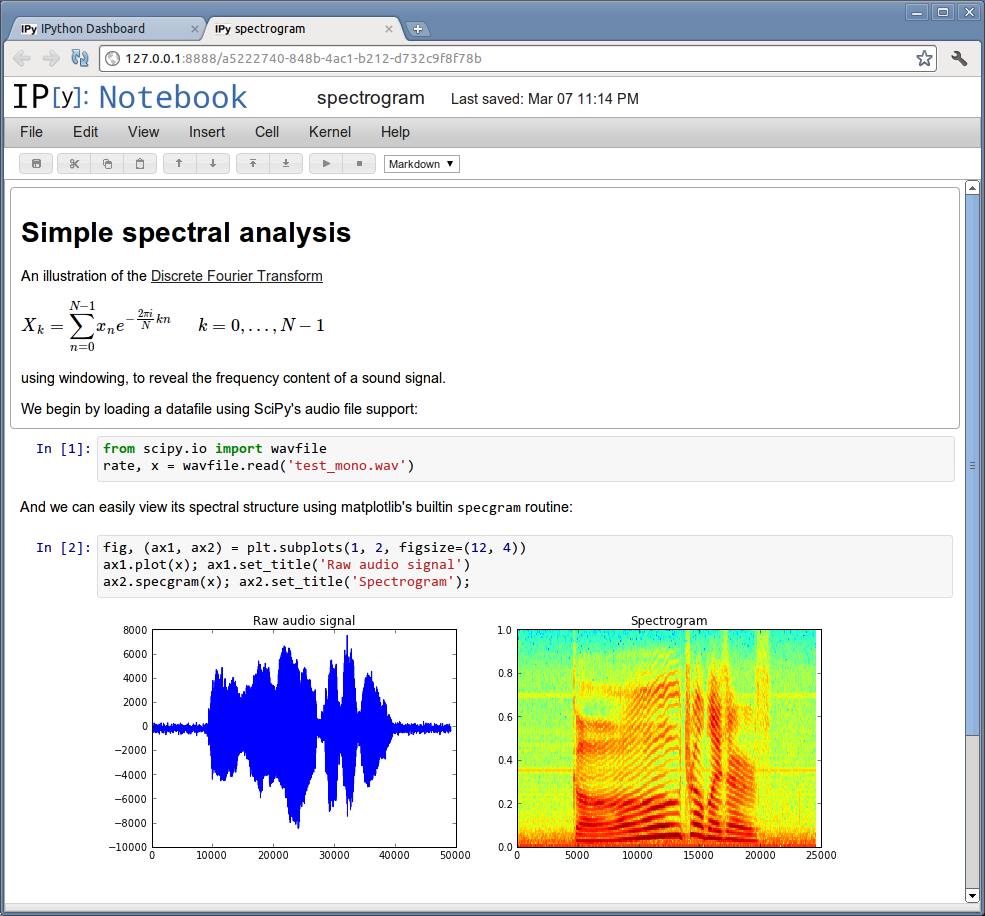
\includegraphics[width=1.0\textwidth]{img/ipython_notebook}
		\caption{An IPython notebook with rich text, mathematical notation, source code and results from executing such code.}
		\label{fig:ipython:notebook}
	\end{figure}
	
	One trend in its community, one that is supported by IPython notebooks, is to make results in publications more reproducible. 
	Instead of publishing a PDF or making a blog post the authors write whole publications as IPython notebooks which then are shared and thus allow everyone to run their source code. 
	Having access to a working copy of the notebook, one can also experiment with it to better understand it, form own conclusions or find errors.
	
	Since it aims to be ``A tool for managing the entire lifecycle of a scientific idea''\footnote{Quoting Fernando Perez in his Scipy 2012 Keynote.}, it also provides parallel computation primitives.
	
	%IPython architecture
	IPython was decomposed into ``execution kernels'', a communication protocol and several front-ends. 
	As each type of component has a defined interface it is possible to implement new specialized components (a new frontend or a new execution kernel) that will integrate with those already implemented.
	
	%Why is it important? I can't imagine designers using it.
	The style of producing notebooks in IPython is one that mixes programming, writing and exploring. 
	This style is also part of a designer's processes. 
	Like a scientist, the designer also has to do exploration of ideas (design ideas in his case), reach conclusions (finalized designs) and share his work with others (fellow designers, clients, friends, blog readers). 
	IPython notebooks, more generally notebooks, are natural tools for exploration.
	IPython notebooks don't provide domain specific functionality for architecture.
	
%Domain-specific IDEs for graphics, games, 3d modeling and Generative Design.
\subsubsection{Processing\cite{reas2007processing}}
	Processing is a programming language and a development environment aimed at ``promoting software literacy in the visual arts and visual literacy within technology''.\footnote{Quoting www.processing.org, 9/Nov/2015.}
	It has an heavy focus on encouraging interaction between its users and so has attracted a big community.
	
	Processing makes it easy to start writing programs that produce visual output. 
	The only step required to start using it is the download and installation of one of its releases. 
	After installation one can start the \ac{pde} and start writing a new program, or a \emph{sketch} as it is referred within Processing. 
	Its website also provides a set of tutorials to help users learn how to use it.
	
	Being aimed at producing visual output and given its success by the size of its community, it makes sense to analyze it.
	
	We start by analyzing its programming language, then move to its development environment and finish by evaluating it against \emph{our learnable programming principles}.
	
	%\subsubsubsection{Processing's programming language}
	Processing's programming language aims to provide Java-style programming while making it easy to quickly write functioning programs. 
	
	Every program written in Processing is called a \emph{sketch}. 
	All \emph{sketches} are stored in a \emph{sketchbook}.
	
	A \emph{sketchbook} has a set of resources, such as images or videos, that can be used by \emph{sketches} that are stored in it.
	
	A \emph{sketch} is a list of instructions to draw something. 
	Some examples of instructions are drawing a shape, like a rectangle, changing the colors used for drawing lines or filling shapes, and changing the color of the background.
	
	To simplify the \emph{sketch}, named functions can be defined to group instructions. 
	These functions can then be used as instructions throughout the rest of the \emph{sketch}.
	
	A \emph{sketch} can be a static sketch or a dynamic sketch. 
	A static sketch produces a static image while a dynamic sketch produces a series of images. 
	A dynamic sketch includes at least a list instructions of what to do to draw each image; it can also include instructions of what to do to respond to input from the viewer of the \emph{sketch}.
	
	\lstset{ %
		basicstyle=\tt\small,
		numbers=left,
		numberstyle=\tt\small,
		frame=lines,
	}
	\begin{lstlisting}[caption={A simple Processing sketch.},label={lst:simple:processing}]
//Hello mouse.
void setup() {
	size(400, 400);
	stroke(255);
	background(192, 64, 0);
}

void draw() {
	line(150, 25, mouseX, mouseY);
}
	\end{lstlisting}
	
	The code in \ref{lst:simple:processing} shows a simple \emph{sketch} with the typical \emph{sketch} structure. 
	The \emph{sketch} draws a white line from one point to the mouse's position. 
	It defines the function ``setup'' and  ``draw'' that specify how to setup for drawing and specify how to draw each image. 
	The ``setup'' is run once when the sketch is started and ``draw'' is repeatedly run afterwards.
	
	%\subsubsubsection{Processing's programming environment}
	The \ac{pde} is shown in figure \ref{fig:proc:dev:env}. 
	It is a code editor dedicated to writing Processing \emph{sketches}. 
	It supports common tasks performed while writing them such as running the currently opened \emph{sketch}, adding/creating resources to the \emph{sketchbook} or exporting \emph{sketches} as executables for several platforms. 
	It also enables the use of multiple files to structure the \emph{sketch's} code.
	
	The \ac{pde} only aims to be an introductory environment for programming. 
	It doesn't replace an advanced software development \ac{ide}.
	
	\begin{figure}
		\centering
		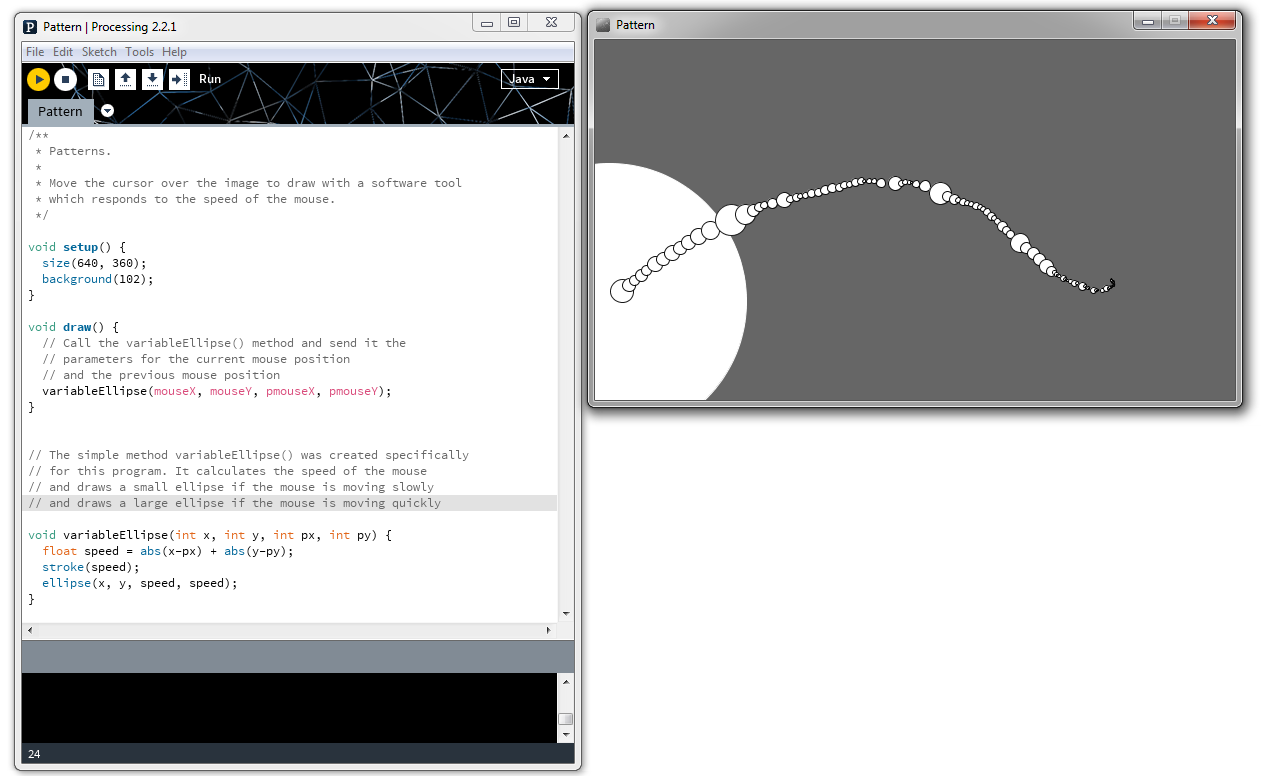
\includegraphics[width=1.0\textwidth]{img/proc_dev_env}
		\caption{On the left: The \ac{pde} displaying an example \emph{sketch} while it is being run. On the right: The drawing window to which the \emph{sketch's} instructions are applied.}
		\label{fig:proc:dev:env}
	\end{figure} 
	
	%\subsection{Processing vs Programming for Everyone}
	%This is a comparison with Java. It can be seen as a limitation.
	Looking at the code in \ref{lst:simple:processing} also reveals the language's resemblance with Java. 
	The same code fragment in Java declares two methods named ``setup'' and ``draw'' that return nothing; both methods belong to whatever class they happen to be inside of; and both have a list of statements to be executed sequentially when they are invoked. 
	Processing's instructions, functions and sketches map to Java's statements, methods and classes.
	%Classes inside sketches are mapped into inner classes.
	
	%Describe what the language and the environment lack to improve the programming experience for its users and uses (arts). 
	%Describe how it is just a quick start package for graphics programming in Java. 
	%Describe how the environment not only lacks a debugger but also doesn't give proper error messages when something fails and doesn't provide other ways to follow the program execution.
	%Describe how the environment fails to be a better environment than those used in industry software production (like Eclipse).
	%Describe how its users are required to look for documentation when programming.
	%Describe how little feedback the environment provides. E.g. he has to run the sketch to see if it compiles and runs as he expects. This blocks creation by reaction.
	%Describe how trying to hide Java doesn't make it a better language for learning or producing art. For doing more advanced things, Processing still requires the programmer to know Java; why not learn Java straight away? Processing tries to hide Java's metaphors, its objects; bad idea. (Scala does a better job, I suppose)

\subsubsection{DesignScript\cite{aish2012designscript}}
	%TODO collections can be used everywhere one thing can be used
	%TODO handling collections (replication guides, etc)
	DesignScript is a programming language that was designed to suit the needs of architecture related design and engineering.
	
	%DesignScript programming paradigms
	DesignScript uses concepts from multiple programming paradigms like object-oriented, functional and associative programming. 
	Entities have properties that can be either data or functions like in object-oriented languages; functions' most important role is to take some input and produce some output without producing side-effects like in functional languages; and dependencies among variables are retained like in associative languages.
	
	It supports both imperative (following instructions step-by-step) and associative (propagating changes in a dependency graph) control flows. 
	The programmer can choose to have portions of the code following one type of control flow and other portions following the other.
	
	%DesignScript primitives
	Being a domain-specific language for architecture, DesignScript includes not only primitives to make building 3d models but also operations from the rest of the architecture process such as energy related analysis and architectural elements (like creating or editing \ac{bim} families).
	%\emph{It may be better to provide a list of example primitives and operations.}
	
	Having modeling primitives close to those normally used in architecture software and combining several programming paradigms allows the designer to draw from knowledge about architecture modeling while empowering him to express the processes in which those primitives are used.
	
	%DesignScript editor(s)
	Editing DesignScript programs can be done either by writing or by creating a graph. 
	The graph is a more natural representation of the dependency graph among the variables of the program when the associative paradigm is being used; it can also be viewed as a data-flow graph. 
	The written representation of DesignScript is a sequence of statements that specify the relationship between a variable and other variables; defining functions, using the imperative paradigm and reassigning variables is also possible; features that are less encouraged by a graph.
	
	DesignScript is used in several environments. 
	These include a textual editor in Autodesk AutoCAD (Figure \ref{fig:ds:autocad}), a dedicated graph editor called DesignScript Studio (Figure \ref{fig:ds:dsstudio}) and later Dynamo (Figure \ref{fig:ds:dynamo}). 
	Both DesignScript Studio and Dynamo use graph based program editing.
	
	\begin{figure}
		\centering
		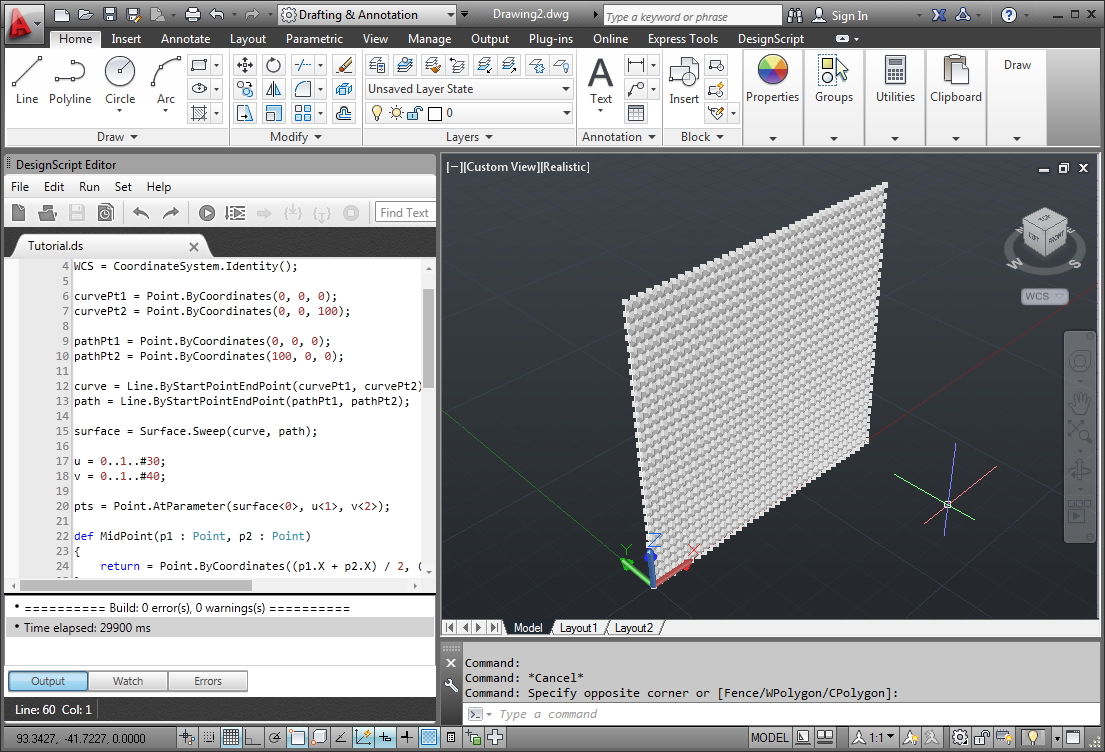
\includegraphics[width=1.0\textwidth]{img/ds_autocad}
		\caption{A DesignScript program being edited in a special text editor inside AutoCAD. This text editor provides auto-complete and a debugger.}
		\label{fig:ds:autocad}
	\end{figure} 
	
	\begin{figure}
		\centering
		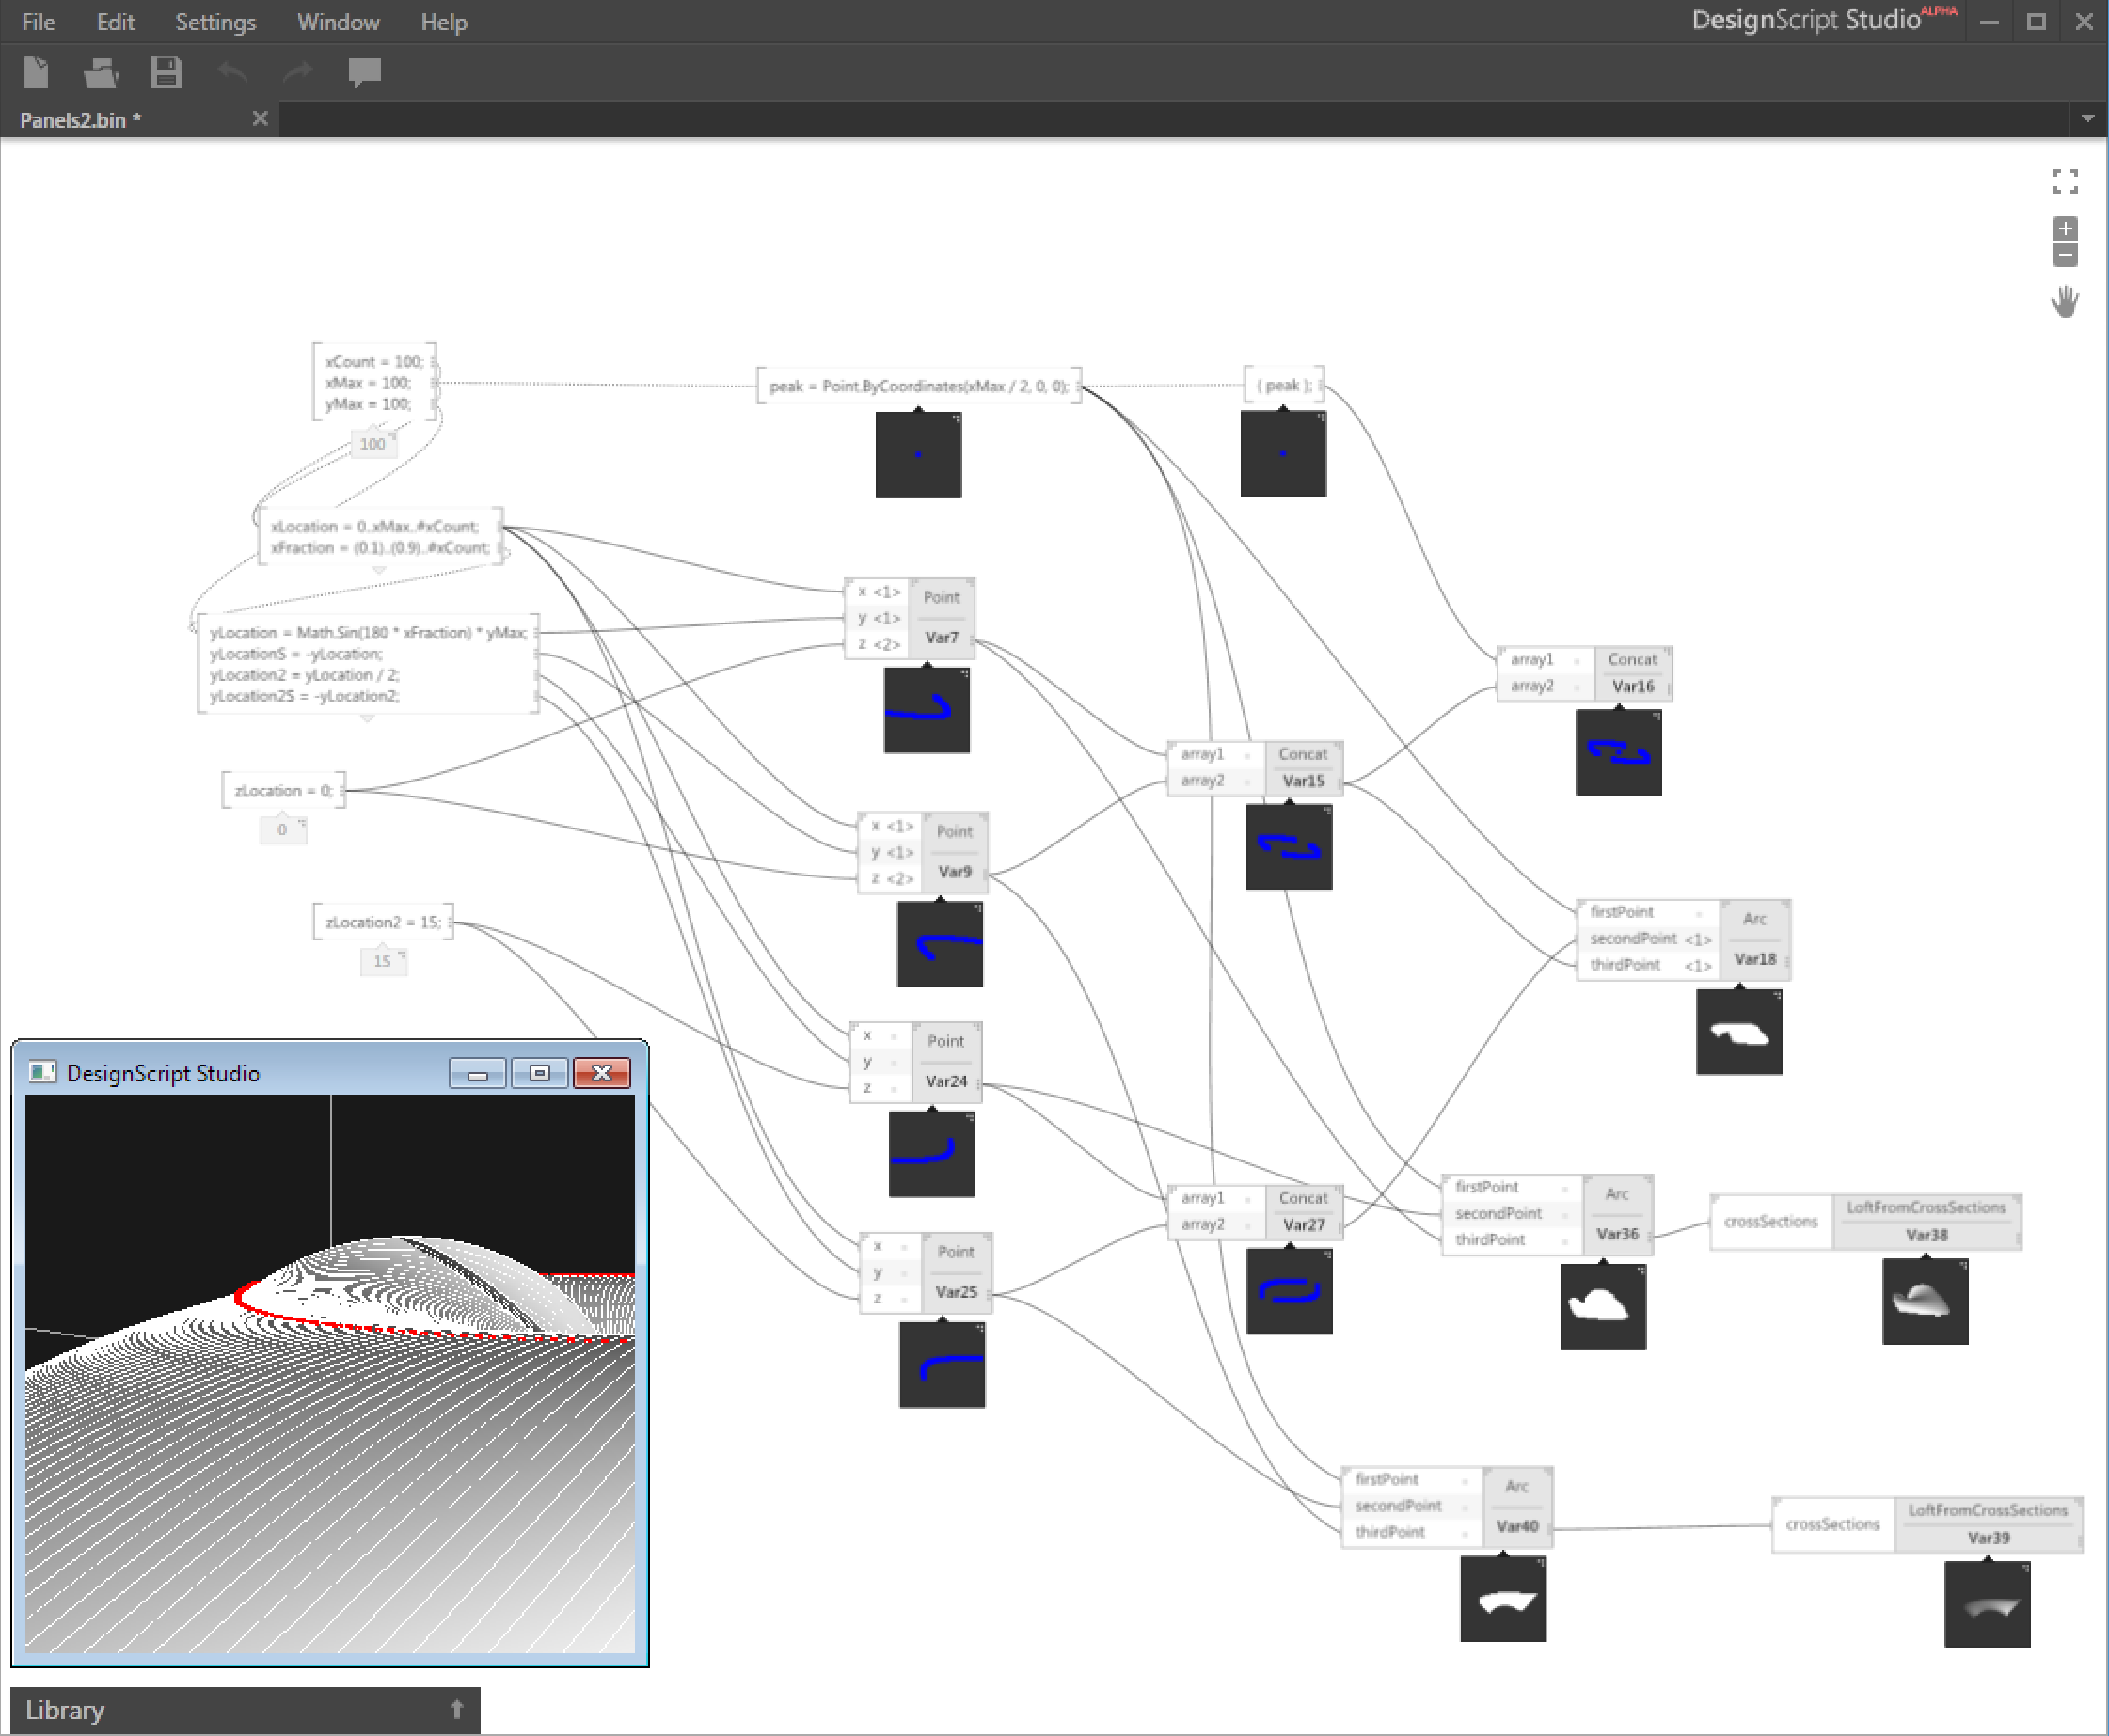
\includegraphics[width=1.0\textwidth]{img/ds_dsstudio}
		\caption{A DesignScript program as a graph in DesignScript Studio. Each node can display a preview of its results. To the bottom left corner is a preview of the whole program results and a folded library tab. The library tab contains everything that can be used in the program.}
		\label{fig:ds:dsstudio}
	\end{figure} 
	
	\begin{figure}
		\centering
		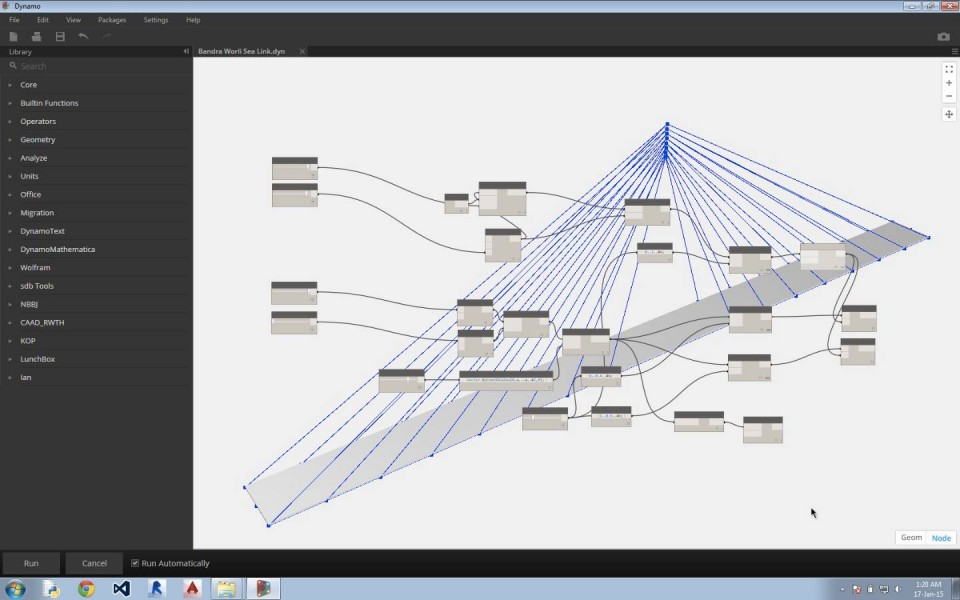
\includegraphics[width=1.0\textwidth]{img/ds_dynamo}
		\caption{Another DesignScript program as a graph in Dynamo. Like in DesignScript Studio a preview of the result of the program is displayed. A contrast is that there is only one preview ``canvas''; the preview from selected nodes is highlighted.}
		\label{fig:ds:dynamo}
	\end{figure} 
	
	Debugging DesignScript programs depends on the environment being used. 
	The textual environment allowed to follow the execution of the program step-by-step while also supporting watches and breakpoints. 
	The graph based environments allow highlighting and listing results of each node. 
	Both the textual and the graph based environments provide a preview of the execution of programs.
	
	%Editing a DesignScript program is usually done in its dedicated development environment. DesignScript development environment provides auto-complete and debugging capabilities both of which are common features among programming environments.
	
	%DesignScript history
	DesignScript was later used as the scripting language of DynamoBIM, integrated with Autodesk Revit, where programs are edited as data-flow graphs. 
	DesignScript was also integrated into Autodesk AutoCAD. 
	A standalone node-based DesignScript editor was also made, it was called DesignScript Studio.
	
	%It is a multiple paradigm language supporting both imperative and associative programming. At any given point in a DesignSript program, the execution is either being controlled imperatively(following instructions step-by-step) or associatively(propagating changes in a dependency graph). It also uses object-oriented concepts; entities are objects with properties and methods; each object has it's own properties and methods;
	%
	%One way DesignScript tries to succeed is to integrate various ways of modeling into the design process. These various ways of modeling are direct-manipulation mode present in any 3d modeling application, the associative mode present in many visual programming environments and the 

\subsubsection{Rosetta\cite{de2012modern}}
	Rosetta is a platform for \ac{gd}.
	It grew from the desire to give the freedom to designers using the \ac{gd} to write their programs using the programming language they want and to easily switch where it takes effect.
	
	Its authors argue that most environments for \ac{gd}, developed for a specific \ac{cad}, don't provide portability of programs developed inside them.
	They also argue that \ac{vpl}s, based on data-flow graphs, don't provide good abstraction mechanisms; programs on such languages are therefore hard to understand and modify.
	
	It is also stated that general purpose programming languages, like C, C++, Java and C\#, don't provide domain-specific abstractions from \ac{gd} and so they are inadequate.
	
	A survey of the most used \ac{gd} systems showed that the most popular \ac{tpl}s for \ac{gd}, like AutoLisp, RhinoScript, and GDL, are old, provide little domain-specific features and make it difficult to define them.
	It also showed that \ac{vpl}s for \ac{gd}, like Grasshopper and GenerativeComponents, enforce a very restricted programming paradigm and programs scale poorly with size and complexity, making them suitable only for small throwaway prototypes. 
	It also showed that \ac{cad} applications, being based on direct user interaction and imposing their own programming environments and languages, lock their users to the application's product family and make it difficult to achieve correctness, performance and portability.
	
	The design principles followed by Rosetta are:
	\begin{itemize}
		\item portability (program independence from \ac{cad} applications) (enabling reuse of programs across different \ac{cad} application communities)
		\item parametric elements (don't require designers to manually transform parametric elements into geometric shapes \ac{cad}s understand)
		\item functional operations (operations don't consume their arguments) (don't leak \ac{cad} implementation details into \ac{gd} languages)
		\item dimension independent operations (uniform, predictable treatment of shapes of different dimensions)
		\item algebra of sets (shapes as point sets in three dimensional sets) (support for operations on sets)
		\item algebraic equivalences (to handle support discrepancies of set operations across \ac{cad}s and for optimization)
		\item traceability (between the parts of the program and their results)
		\item immediate feedback (to changes made to the program and its input)
	\end{itemize}
	
	A modern programming environment for \ac{gd} should:
	\begin{itemize}
		\item be pedagogic
		\item provide domain-specific features
		\item provide multiple Programming Languages
		\item provide multiple \ac{cad} applications
	\end{itemize}
	
	Generative Design needs:
	\begin{itemize}
		\item Portability
		\item Mathematical and geometric strictness
		\item Correlation between programs and models
		\item Multiple paradigms and techniques
		\item Modern and pedagogic system
	\end{itemize}
	
	It enables this by providing several ``frontend'' programming languages and several ``backends'' which take the results of the program. 
	The programs written in a ``frontend'' language are compiled into an intermediate language which then translates its semantics to the selected ``backend''.
	
	Some ``frontends'' supported by Rosetta are AutoLisp, Javascript, Racket and Python; some of the supported ``backends'' include Autodesk AutoCAD, Autodesk Revit, Sketchup, Rhinoceros 3D, TikZ and OpenGL.
	
	%Rosetta has been extensively used for teaching programming to architecture students at \ac{ist}. 

\subsubsection{Learnable Programming\cite{victor2012learnable}}
	Writing a program in a programming language can be difficult even if it was designed to be easy to use. 
	When a programming language is coupled with an environment specifically designed for it the programming experience improves drastically. 
	In his essay\cite{victor2012learnable}, Bret Victor described design principles over systems for learning programming.
	
	The programming language and the programming environment are essential parts of the programming experience.
	The programming language allows the programmer to express himself in a clear, specific way; the programming environment allows him to write programs and understand what they actually do.
	
	Programs written in the programming language need to reflect something from the programmer that is useful for programming.
	They should be about things the programmer can identify with (something that he knows); should allow him to talk about different parts of the problem separately; should allow him to bring those parts together; and should be readable.
	
	The environment needs to help understand the meaning of the parts of the program; understand the way the program execution evolves; understand the way the state evolves; assemble parts together; and create new parts from existing ones.
	It should make these things easy to do, after all these can be done by the programmer alone if he is willing to.

\subsection{Moving to the Web}
	Web browsers didn't start as feature-rich and performant as they are now.
	They started as hypertext browsers that made it easier to read hypertext.
	They could display images and text and could jump from page to page by following hyperlinks or following URLs.
	Only with the development of new features and the demand for more performance and features did they slowly get into the shape they are now.

	The number of devices connected to the internet is big enough to say that internet access is almost ubiquitous.
	People no longer have to rely on a single device because many of the things they do on that device can be migrated to the internet as distributed systems.
	If viewed this way, devices can become windows to distributed systems over the internet.
	With such idea people can start to use any device to access those distributed systems.

	There must be a platform to support (as in display) such windows and Web browsers are a good possibility.
	Almost any of these devices have web browsers.
	These not only include the traditional desktop and laptop computers but also the new smartphones, tablets, gaming consoles, smart appliances and the list goes on and on.

	Web browsers enable devices to connect their users to the \ac{www} and in many cases to the rest of the internet, as \ac{www} is often used as an interface to services on the internet.
	Some of those interfaces are as simple as a series of web pages generated by the service as they are used and some are as complex as pages interactively evolving with user input while at the same time exchanging information with many servers.
	Most blogs are examples of the first, technically simple, and most social networking sites are examples of the second, technically complex.
	All of these have forced web browsers to evolve into a performant, feature-rich platform.
	The extent of their performance and features makes them even capable of hosting desktop applications from code editors to video games (without plugins like Adobe Flash).

	And this has caught on.
	More and more people are replacing their desktop applications with web based ones.
	Web browsers are effectively replacing \ac{os}-level applications.
	And this also comes as an advantage for developers as the browser acts an uniform platform across all different devices they want to develop for.

	It is in this time where web browsers are so capable that it becomes possible to develop a \ac{gd} \ac{ide} for the web.

%Inspiration from anything about IDEs.
\subsubsection{LightTable}
	LightTable is an example of a desktop application that uses Web technologies.
	More specifically, it uses node-webkit as its runtime allowing it to use html layout engine for its user interface, to use javascript as its programming language and to use node.js\cite{tilkov2010node} modules.
	LightTable is written in ClojureScript\cite{10.1109/MIC.2011.148}, a subset of Clojure that compiles to Javascript.

	LightTable is a code editor for the Clojure programming language\cite{hickey2008clojure}. 

	%Disclaimer
	%Most of the features described here are only present in LightTable's several experimental versions. 
	%The release version's features are not what matters. 
	%The ideas behind the experiments are.

	%Why is LightTable relevant?
	%As of now, LightTable doesn't seem to be fulfilling its potential.
	LightTable uses the drafting table as its metaphor\footnote{http://www.chris-granger.com/2012/04/12/light-table---a-new-ide-concept/ at Nov/2015.}. 
	The metaphor comes from looking at the way work is done in other fields of engineering, where engineers spread all materials relevant to their work over large tables, from tools to reference information. 
	Instead of displaying the contents of entire files, LightTable divides the code into meaningful units and displays them as small editors spread over the table's surface. 
	In one of its experimental versions, LightTable also supported displaying running programs in the table. 
	Figure \ref{fig:lt:draft:table} shows an example of this metaphor.

	This metaphor has some resemblances to node-based programming environments. 
	The programmer still has think of how to arrange what is on the table.
	What makes it different is allowing to choose what is on the table instead of having everything on it all the time.

	\begin{figure}
	  \centering
	  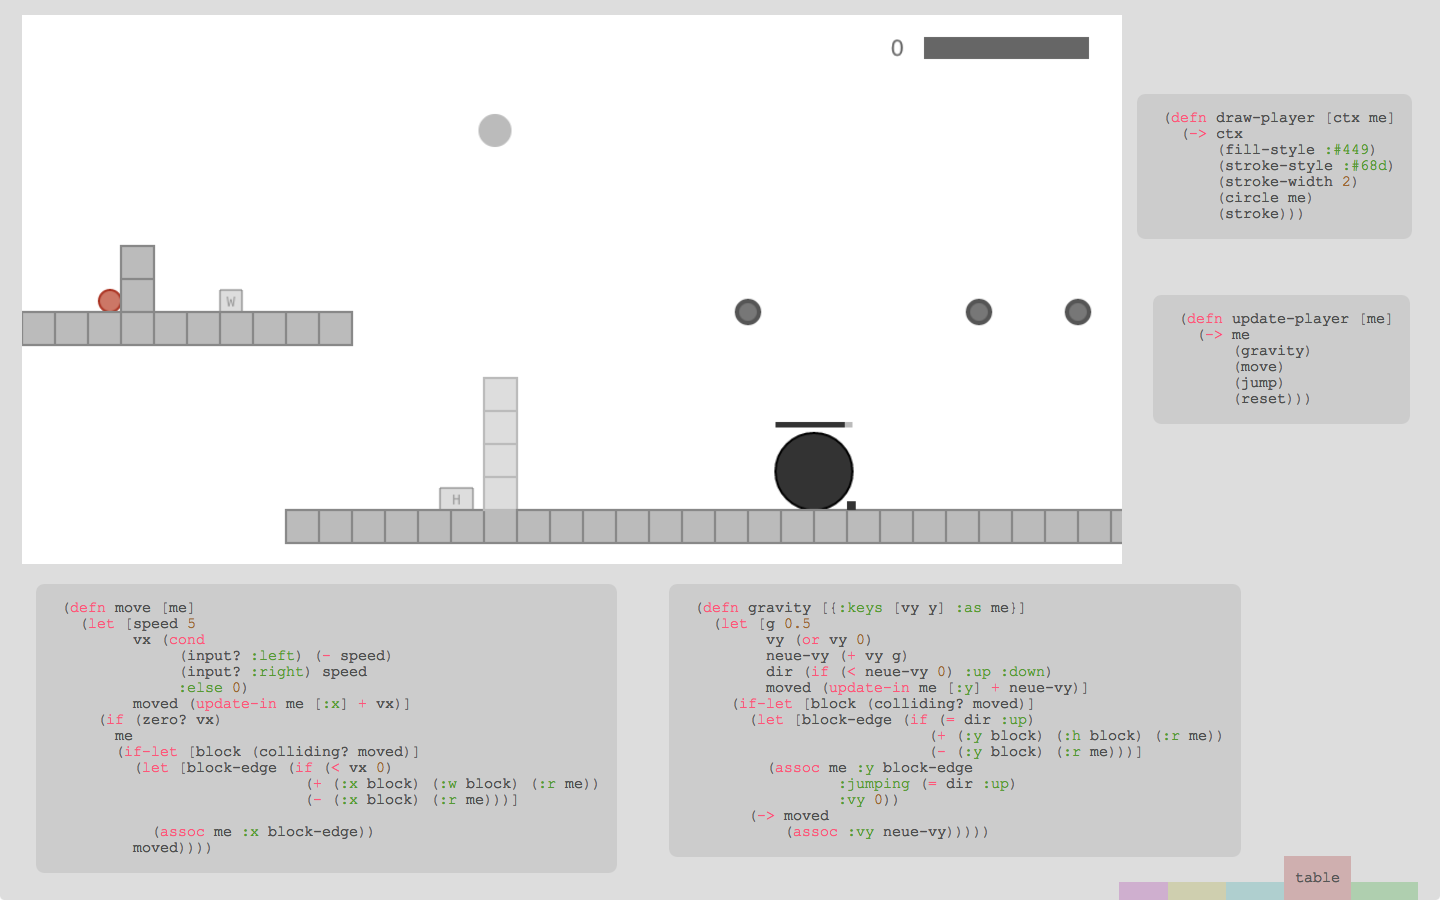
\includegraphics[width=1.0\textwidth]{img/lt_game_example__inv}
	    \caption{A prototype version of LightTable. A game is being run inside it while some of its code is displayed in separate editors.}
	  \label{fig:lt:draft:table}
	\end{figure} 

	%LightTable "function navigation"
	LightTable also helps navigating Clojure code bases.
	In Clojure functions are defined inside namespaces and all Clojure definitions (functions, variables, macros) are stored in text files. 
	Navigating among definitions and the current namespace structure shouldn't get in the way of editing code. 
	To make editing easier, LightTable provides a \emph{namespace browser} that eases finding functions and a \emph{code document} where functions can be added for editing without moving them out of their namespace or displaying entire files where they are defined. 
	Figure \ref{fig:lt:clojure:table} shows an experiment where these two are used.

	\begin{figure}
	  \centering
	  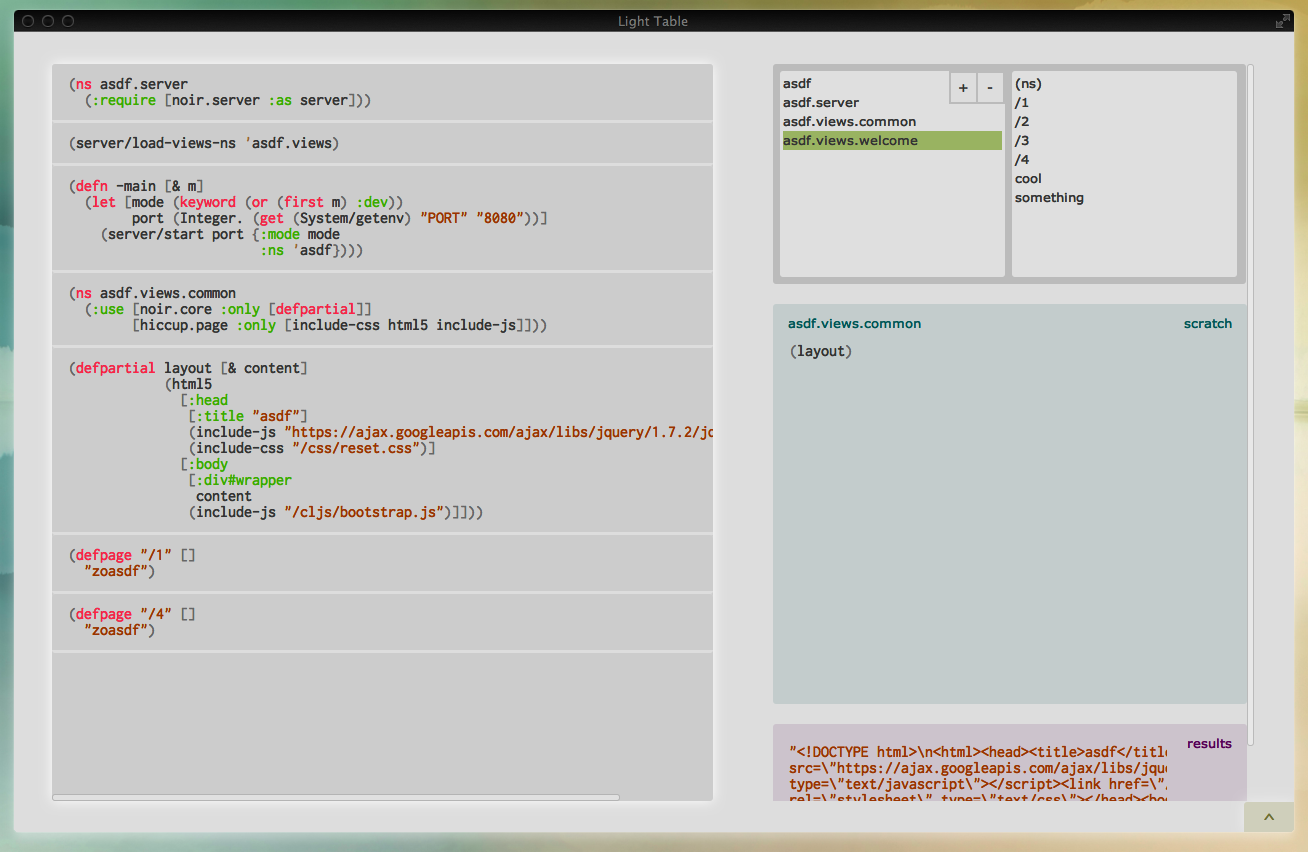
\includegraphics[width=1.0\textwidth]{img/lt_clojure_table__inv}
	    \caption{An experiment showing a \emph{code document} on the left and a \emph{namespace browser} on the top right.}
	  \label{fig:lt:clojure:table}
	\end{figure} 

	%LightTable "variable substitution"
	One interesting functionality of LightTable is its ability to show data flow in a function call. 
	Since the main purpose of a function is to transform its input data into its output data, it helps to see what happens to the data on each step of the function. 
	To achieve this LightTable overlays variable values and return values, respectively, on each variable occurrence and expression of the function. 
	Figure \ref{fig:lt:val:overlay} shows an example of such functionality. 
	This functionality is part of LightTable's \emph{instarepl}.

	\begin{figure}
		\centering
		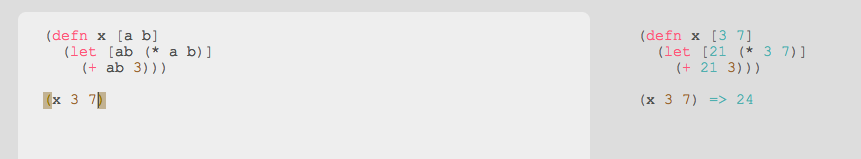
\includegraphics[width=1.0\textwidth]{img/lt_val_overlay__inv}
			\caption{An example of LightTable's value overlaying. The occurrences of the variables \emph{a}, \emph{b} and \emph{ab} were replaced with their values while evaluating the expression \emph{(x 3 7)}; the result of this expression is also overlaid.}
		\label{fig:lt:val:overlay}
	\end{figure}

	The main design pattern used in LightTable is the \ac{bot} pattern. 
	As described by one of its developers\footnote{http://www.chris-granger.com/2013/01/24/the-ide-as-data/ at Nov/2015.}, LightTable can be described as a set of \emph{Objects}, each having a set of \emph{Behaviors} and being tagged with a set of \emph{Tags}. 
	The \emph{Behaviors} describe how an \emph{Object} reacts when events are raised on it. \emph{Tags} are groups of \emph{Behaviors}. 
	When an event is raised on an \emph{Object} both its \emph{Behaviors} and those from its \emph{Tags} are notified.

\subsubsection{OpenJSCAD\cite{openjscad2015site}}
	OpenJSCAD is a javascript application (or rather, an application based on web technologies).
	It aims to provide the same functionality as OpenSCAD but using javascript as a base for its language. 
	Most of OpenSCAD functionality is implemented in OpenJSCAD. 
	Like OpenSCAD, it focuses on creating 3D models for 3D printing (e.g. they are solid).

	To actually model in OpenJSCAD the user has to write a program in either OpenJSCAD's language or OpenSCAD's language.

	It is also possible to import 3D models from files commonly used for 3D printing like STL and AMF files.
	Upon import, the file's content is converted to a jscad program that produces the same model. 
	%(I don't see the point of doing this.)

	OpenJSCAD provides two user interfaces, one command-line interface and one graphical user interface as a web page.
	The first can be used for batch processing (running programs) while the second integrates an editor to edit a program and a 3D view for viewing the results of that program.

	OpenJSCAD's language supports two syntaxes, one based on message passing (or method invoking) and one based on calling functions.
	Both of these syntaxes are already present in javascript. 
	Many operations provided produce a new object and don't change their parameters. 
	This allows us to follow a functional programming paradigm and since there are fewer side-effects to know about it is easier to understand a program written using them.

	A problem that can arise while writing and testing jscad programs is that there is no help on getting the parameters for operations right.
	It will be frustrating to spend more time than acceptable trying to understand why a certain operation is not producing the desired result. 
	This problem is even more relevant when most of the operations have multiple optional parameters and parameters that replace others. 
	Currently the only help available is OpenJSCAD's documentation (a tour on its functionality), the online community around OpenJSCAD and, since javascript is the core of the language, web browsers' javascript developer tools.

	A problem using function call syntax.
	It may not provide the flexibility needed for arranging the code in a easily readable manner. 
	This is especially true if a simple text editor is used. 
	While assigning intermediary results to variables can help ``unnesting'' but it is sometimes inconvenient. 
	On top of this OpenJSCAD is mainly just javascript and so javascript's strange behavior about semicolon insertion is carried over. 

	A good thing about being based on javascript is the possibility of using higher order functions for modeling tasks.
	Examples of this advantage can be found in \textbf{leitao abstract geometry n high order programming}.

	%Some functions in OpenJSCAD and their parameters.
	%function parameters result 
	%Each primitive has a lot of options on how to call it.
	%Its possible to round the edges of polyhedral primitives.
	%Non-polyhedral primitives are always converted to polyhedral approximations.

%----------------------------------------------------
%NAVarchitecture
\section{Architecture (2/3pgs)}

\subsection{Decomposing the problem}
	To better understand how to solve the problem of helping to make programs for GD, we decomposed it into several parts that can be more or less thought about and solved separately.
	
	\paragraph{The programming language}
	One part that has to be set is \textbf{what is the language} used to make the programs.
	This aspect involves things like what control flow mechanisms are available, whether side-effects exist or not, and what is the syntax for each component of the language.
	It deals with how the language works.

	\paragraph{Help when writing and reading}
	Another part is the \textbf{amount of help, documentation or reaction} the system has to support the user while he is thinking about and making the program.
	In the light of \cite{victor2012learnable}, the system should have good answers to the questions proposed on what is a good programming environment.

	\paragraph{Primitive operations}
	Another part is the \textbf{implementation of primitives} of the language like constructive solid geometry, lofts, sweeps and many other 3D modeling operations.
	Without them architects won't be able to make any Generative Design.
	One thing to keep in mind is that these operations have to be translated into other tools used in architecture.

	\paragraph{Documenting programs}
	Other part is how the system lets users \textbf{document their programs}. 
	It is normal to forget how some part of the program works and so documentation is needed (or anything that is faster to understand than interpreting the program manually).
	The system could support having drawings juxtaposed to the program in addition to previews of results like those present in DesignScript Studio, Dynamo and Grasshopper. 
	It will also be useful to look at how current programming languages are usually documented. 

	\paragraph{Persisting programs}
	Other part is the \textbf{persistence of programs} between usage sessions, in cases the system crashes or even across multiple devices.
	In case of persistence between sessions, the user can close the browser or the tab at any moment, it would be useful to keep record of the current program in some way. 
	In case of persistence in case of crashes, if the user program itself crashed the page it should not be executed immediately to allow its retrieval or edition (as it could crash the page again). 
	With persistence of programs also comes the need for holding different versions of the same program. 
	These become useful as the user makes changes and wants to look back in time for some reason. 
	Maybe because he did not anticipate the need for something he deleted or maybe because he wants to see how his programs have progressed.

	\paragraph{Passing results on}
	Other part is the way programs can be \textbf{applied to other modeling applications} used by architects.
	Without a way to do this the system is rendered useless as it can hardly be integrated into the architect's normal process. 
	Rosetta uses the concept of selecting a backend, a specific interface to a modeling application. 
	After selecting a backend for a modeling application, Rosetta connects to it and results of running the program are passed to the application. 
	The system could connect to Rosetta which would then connect to the application. 
	This approach requires the setup of a communication channel between the browser where the system is running and Rosetta. 
	The system could alternatively use a language that Rosetta already supports. 
	When the user wants to pass the result of the program to the application he only has to select the desired backend and run the program inside Rosetta.

	%It should enumerate the various aspects of concern to be considered while making the solution. It may as well provide some alternatives to some aspects that are already known. These alternatives can refer to products already available.

\subsection{General Architecture of the Solution}
	Taking into account the aspects described above a version of the architecture of the solution was made.
	
	The center of the \ac{ide} is composed by an editing environment, where source code is edited, and a visualizer, where results of running a program are visualized in 3D.
	Both of these are hosted within the web browser of the user and like so after the \ac{ide}'s web page is served to the browser it is no longer dependent on external computers.
	
	As starting ideas for features that will help users understand programs there is highlighting the 3D objects in the resulting scene that were ``affected'' by a part of the program and also letting users change the value of constants in source code using widgets, like sliders, to see their effects on results.
	
	Interacting with programs and their results will only be possible if the \ac{ide} can display results or update them fast enough so a great part of our work will be in making sure it is.
	This may involve compromising the quality of the 3D scene that represents the results to get faster.
	
	Since there is no dependency on other machines, supporting program persistence and allowing the results of programs to get to other software are limited to what a web browser can do.
	Since web browsers allow some local storage to web pages, programs can be persisted there, at least temporarily.
	On the side of getting results into other software, without communication with the outside we are limited to either using a programming language supported by Rosetta or exporting to a widely supported file format.
	
	The architecture of the editing environment and the visualizer together with the program persistence module and the export module can be visualized in Figure \ref{fig:gen:sol}.
	
	\begin{figure}
		\centering
		\includegraphics[width=1.0\textwidth]{img/gen_sol}
		\caption{A diagram of the architecture of the solution. Rectangles represent components, dashed rectangles represent where components will run and lines represent communication between components.}
		\label{fig:gen:sol}
	\end{figure}	

%----------------------------------------------------
%NAVevaluation
\section{Evaluation (1/2pgs)}
	To evaluate an \ac{ide} for \ac{gd} we will have to look at three different areas:
	its performance, its user experience or usability and its Generative Design capability.
	
	\paragraph{User experience / Usability}
	For the system to be useful its users have to be able to use it.
	To assess that this is true we will do user testing.
	
	The tests will follow the line of asking users to complete a small \ac{gd} programming task followed by giving their opinion on how the usage experience went.
	We can complement those with questionnaires on the same subject and also by recording the usage sessions (which will also allow users to pinpoint their opinions).
	
	Only the editing environment will be tested this way since it is the only component that is used directly by architects.
	
	\paragraph{Generative Design capability}
	The variety of results that can be made using the system is also important for its evaluation.
	The more \ac{gd} examples it can produce the better it is suited for use in a real-world scenario.
	A way to show how much variety of results it can make is to describe several examples that give glimpses of that variety.
	
	\paragraph{Performance}
	The performance will have to be evaluated but more importantly its perceived performance, or responsiveness, will also be evaluated.
	As the \ac{ide} will be used by people, it is important that the interface responds quickly;
	in this case it will matter how much time it takes to see the changes made to a program appear on a view of its results.
	
	Performance will be evaluated by benchmarks to compare our solution against other \ac{gd} \ac{ide}s and also by measuring the frame rate of the viewer.
	The first measures raw performance and the second measures responsiveness.

\subsection{Proof-of-concept Prototype}
	A small prototype has been assembled to test the concept of a \ac{gd} environment in the browser.

	Like shown in figure \ref{fig:proto:3d:p:editor}, this prototype consists in a web page with a text editor and a 3D view.

	\begin{figure}
	  \centering
	  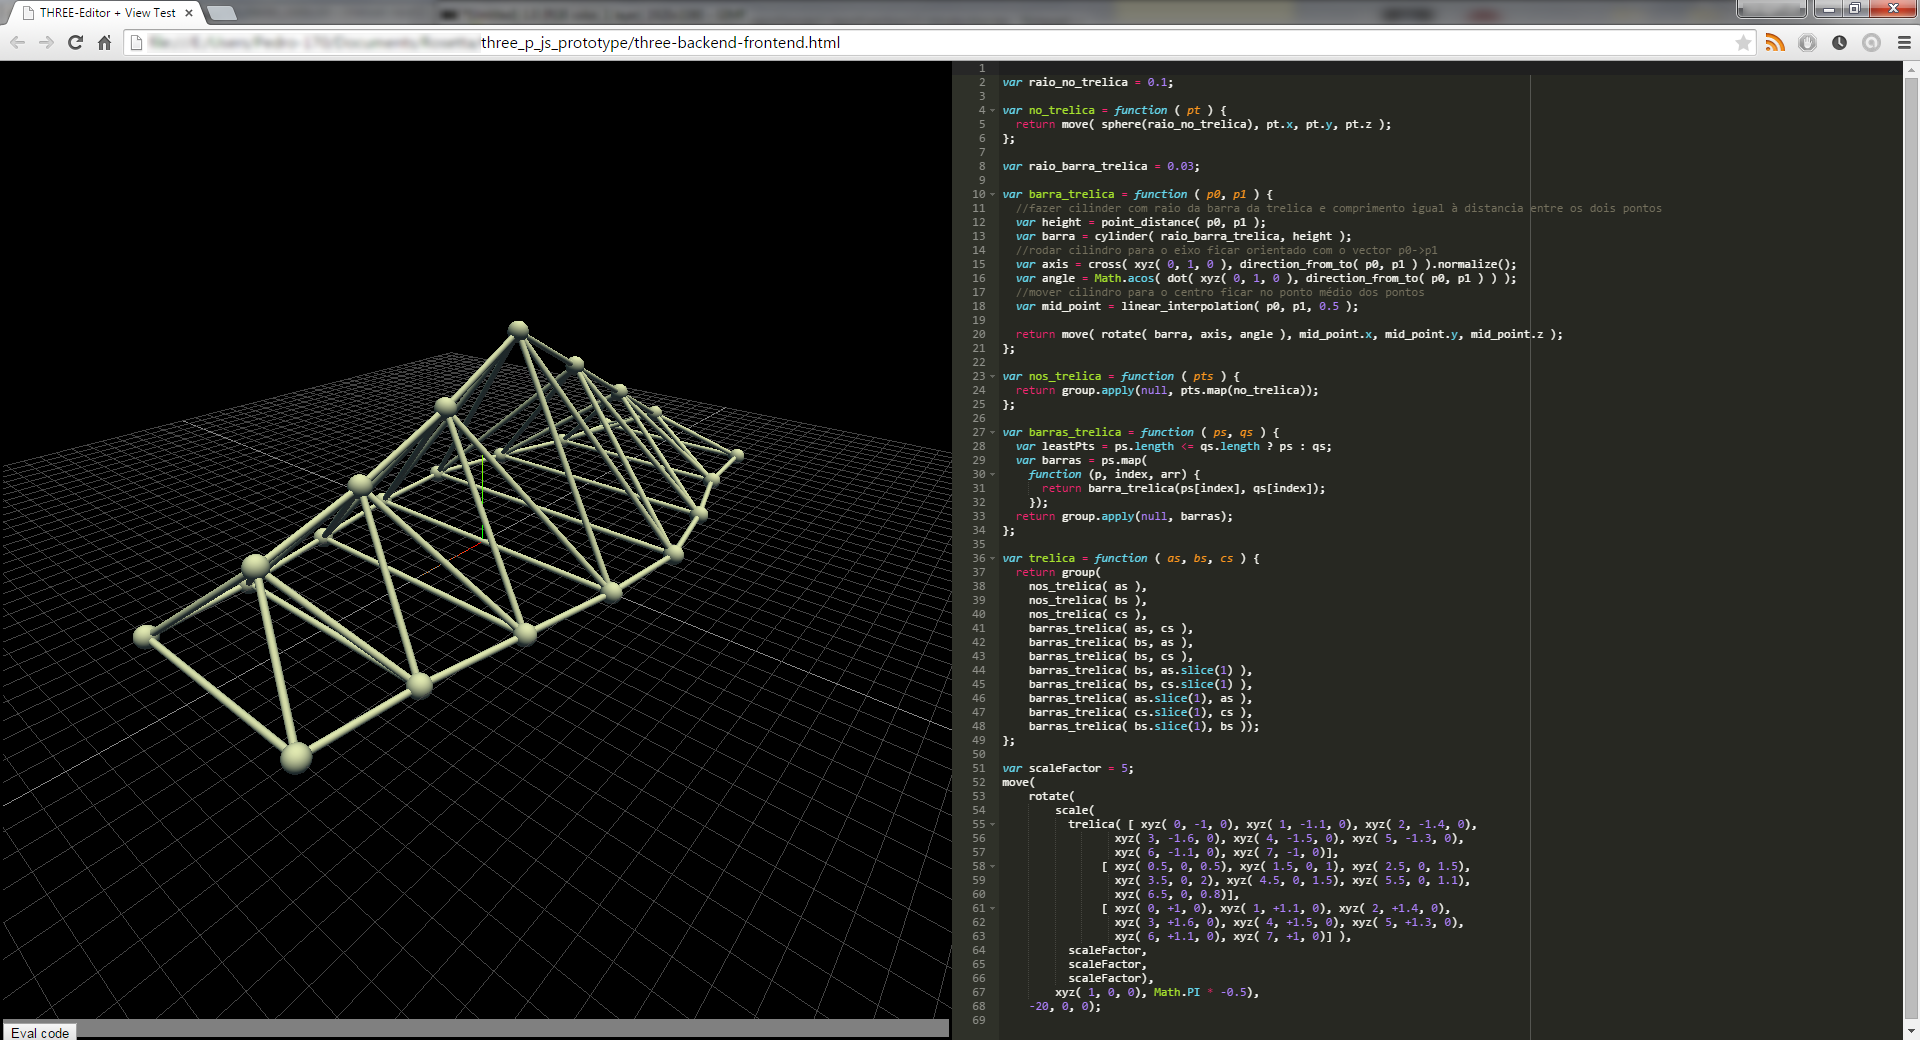
\includegraphics[width=1.0\textwidth]{img/proto_3d_p_editor}
	    \caption{The proof-of-concept prototype generating a truss. The right half contains the program used to generate the truss and the left half contains an interactive view of generated truss.}
	  \label{fig:proto:3d:p:editor}
	\end{figure} 

	The results of running the program inside the text editor are displayed through the 3D view. 
	When the program's text changes, it is rerun to reflect the changes in the 3D view. 
	This enables the prototype to provide immediate feedback to changes as long as they introduce visual changes to the result.

	The user can interact with the 3D view as if it contained a turntable.

	The programming language that is run by the prototype is javascript with several functions added to produce 3D primitives (such as cubes or cylinders) and to manipulate those primitives (such as moving or grouping).

	The prototype is accompanied with example programs which were used to demonstrate it to a small group of potential users.

	The example programs try to emphasize functional programming techniques like using higher-order functions and minimal use of side-effects.

	The overall feedback from the potential users was positive (they wanted to see it on a real application).

	The prototype is implemented using HTML, javascript, CSS and also two javascript libraries; the first, Ace\footnote{http://ace.c9.io/}, provides the text editor and the second, THREE.js\footnote{http://threejs.org/}, provides a high-level interface with WebGL rendering.

	With its naive implementation, the use of the prototype has already made clear one problem: always trying to run a program while it is being changed can lead to poor responsiveness or even permanent lockup of the interface.
	The usual cause being the increasing complexity of the program or the presence of infinite loops in the program. 
	This problem will have to be addressed in order to have a usable interface. 
	Some alternatives to solve the problem could be running the program asynchronously and retrieving the results afterwards or instrumenting the program so it could be run interleaved with interface handling and stopped if necessary.

%----------------------------------------------------
%NAVschedule
\section{Schedule}
	The schedule for the work concluding the thesis is presented in Figure \ref{fig:schedule}.
	It has high-level tasks to convey the overall distribution of work for the thesis.
	
	\begin{figure}
		\centering
		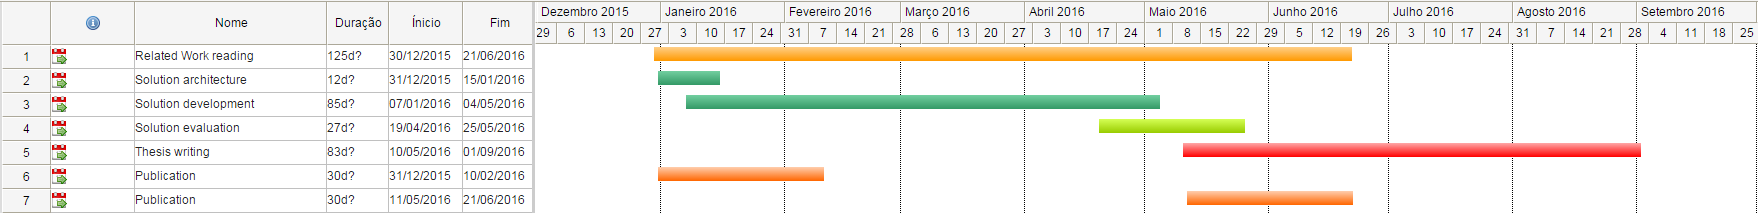
\includegraphics[width=1.0\textwidth]{img/schedule}
		\caption{This chart shows the overview of the work distribution.}
		\label{fig:schedule}
	\end{figure}
	
	The editing environment and the visualizer are the components where must implementation work is since they are the central part of the architecture.
	The implementation of program persistence and result exportation will be in the background.
	As these implementation tasks are complex, they need to be further decomposed.
	
	During implementation we will test both user experience and performance of the system as part of its evaluation.
	
	Close to the end of the implementation we will start to assemble the thesis document and its defense.
	We will be writing parts of the document as candidates to publication in Architecture and Programming conferences.
	(Themes being results and reasons of our work.)
	
	Some work as already been done.
	The proof-of-concept prototype is part of that work, more specifically part of the work on the editor.
		
	

%----------------------------------------------------
%NAVconclusions
\section{Conclusions}
	People making \ac{gd} need an \ac{ide} that is different from those used in software development. 
	Most of the time their programming projects are much simpler than the typical software development project.
	They also don't have as much programming knowledge as software developers.
	With this in mind it becomes clear that software development \ac{ide}s don't fit their needs.
	
	\ac{ide}s like Impromptu, IPython, Processing, DesignScript and Rosetta are examples of \ac{ide}s for programming purposes other than software development.
	They drop most of the functionality from software development \ac{ide}s (like Visual Studio or Eclipse) keeping only what is useful for beginners and add new functionality that will help them while programming for their specific purposes.
	
	With the current state of web browsers it has become possible to host applications inside web pages. 
	Applications that in the past could only be executed by running a native executable can now be moved to web pages.
	LightTable and OpenJSCAD are examples of it.
	
	With the need for a different \ac{ide} for people doing \ac{gd} and the possibility of running applications in the browser, it is not only possible to build an \ac{ide} for \ac{gd} in the web browser but it is also advantageous for users.
	With it, they can quickly open up a web browser on its web page, start to write down their \ac{gd} ideas and immediately run them.
	
	To have a working \ac{ide} for \ac{gd} in the browser there need to be at least two components, a source code editor and a visualizer.
	This way people will be able to make programs and see their results with just a web browser.
	
	Special care will have to be taken to make sure that the user experience is good. 
	A particular element in making it is the overall responsiveness of the user interface and other is the amount of primitives available for \ac{gd}.
	
	In the future, a better solution for storing the programs users make and for running them in \ac{cad}s may be explored.
	
%----------------------------------------------------
%NAVappendix
\newpage
\appendix
\section{Appendix}
\label{sec:attachments}

%----------------------------------------------------
%NAVacronyms
\begin{acronym}
	\acro{api}[API]{application programming interface}
	\acro{ide}[IDE]{integrated development environment}
	\acro{pde}[PDE]{Processing development environment}
	\acro{bot}[BOT]{Behavior-Object-Tag}
	\acro{bim}[BIM]{Building Information Model}
	\acro{ist}[IST]{Instituto Superior Técnico}
	\acro{gd}[GD]{Generative Design}
	\acro{repl}[REPL]{Read-Eval-Print-Loop}
	\acro{cad}[CAD]{Computer-Aided-Design}
	\acro{tpl}[TPL]{Textual Programming Language}
	\acro{vpl}[VPL]{Visual Programming Language}
	\acro{www}[WWW]{World Wide Web}
	\acro{os}[OS]{Operating System}
	\acro{oop}[OOP]{Object Oriented Programming}
\end{acronym}

% 
% Bibliography
% 
\bibliographystyle{plain} 

% replace example.bib with your .bib
\bibliography{report} 

\end{document}